\documentclass[xcolor={dvipsnames}]{beamer}
%\usepackage[utf8]{inputenc}
%\usetheme{Madrid}
\usetheme{CambridgeUS}
\usecolortheme{}

%-------------------------------------------------------------------------------
%          -Packages nécessaires pour écrire en Français et en UTF8-
%-------------------------------------------------------------------------------
\usepackage[utf8]{inputenc}
\usepackage[french]{babel}
\usepackage[T1]{fontenc}
\usepackage{lmodern}
\usepackage{textcomp}

%-------------------------------------------------------------------------------

%-------------------------------------------------------------------------------
%                          -Outils de mise en forme-
%-------------------------------------------------------------------------------
\usepackage{hyperref}
\hypersetup{pdfstartview=XYZ}
\usepackage{enumerate}
\usepackage{graphicx}
%\usepackage{multicol}
%\usepackage{tabularx}

%\usepackage{anysize} %%pour pouvoir mettre les marges qu'on veut
%\marginsize{2.5cm}{2.5cm}{2.5cm}{2.5cm}

\usepackage{indentfirst} %%pour que les premier paragraphes soient aussi indentés
\usepackage{verbatim}
%\usepackage[table]{xcolor}  
%\usepackage{multirow}
\usepackage{ulem}
%-------------------------------------------------------------------------------


%-------------------------------------------------------------------------------
%                  -Nécessaires pour écrire des mathématiques-
%-------------------------------------------------------------------------------
\usepackage{amsfonts}
\usepackage{amssymb}
\usepackage{amsmath}
\usepackage{amsthm}
\usepackage{tikz}
\usepackage{xlop}
\usepackage[output-decimal-marker={,}]{siunitx}
%-------------------------------------------------------------------------------

%-------------------------------------------------------------------------------
%                  -Nécessaires pour écrire des formules chimiquess-
%-------------------------------------------------------------------------------

\usepackage[version=4]{mhchem}

%-------------------------------------------------------------------------------
%                    - Mise en forme 
%-------------------------------------------------------------------------------

\newcommand{\bu}[1]{\underline{\textbf{#1}}}


\usepackage{ifthen}


\newcommand{\ifTrue}[2]{\ifthenelse{\equal{#1}{true}}{#2}{$\qquad \qquad$}}

\newcommand{\kword}[1]{\textcolor{red}{\underline{#1}}}


%-------------------------------------------------------------------------------



%-------------------------------------------------------------------------------
%                    - Racourcis d'écriture -
%-------------------------------------------------------------------------------

% Angles orientés (couples de vecteurs)
\newcommand{\aopp}[2]{(\vec{#1}, \vec{#2})} %Les deuc vecteurs sont positifs
\newcommand{\aopn}[2]{(\vec{#1}, -\vec{#2})} %Le second vecteur est négatif
\newcommand{\aonp}[2]{(-\vec{#1}, \vec{#2})} %Le premier vecteur est négatif
\newcommand{\aonn}[2]{(-\vec{#1}, -\vec{#2})} %Les deux vecteurs sont négatifs

%Ensembles mathématiques
\newcommand{\naturels}{\mathbb{N}} %Nombres naturels
\newcommand{\relatifs}{\mathbb{Z}} %Nombres relatifs
\newcommand{\rationnels}{\mathbb{Q}} %Nombres rationnels
\newcommand{\reels}{\mathbb{R}} %Nombres réels
\newcommand{\complexes}{\mathbb{C}} %Nombres complexes


%Intégration des parenthèses aux cosinus
\newcommand{\cosP}[1]{\cos\left(#1\right)}
\newcommand{\sinP}[1]{\sin\left(#1\right)}

%Fractions
\newcommand{\myfrac}[2]{{\LARGE $\frac{#1}{#2}$}}

%Vocabulaire courrant
\newcommand{\cad}{c'est-à-dire}

%Droites
\newcommand{\dte}[1]{$(#1)$}
\newcommand{\fig}[1]{figure $#1$}
\newcommand{\sym}{symétrique}
\newcommand{\syms}{symétriques}
\newcommand{\asym}{axe de symétrie}
\newcommand{\asyms}{axes de symétrie}
\newcommand{\seg}[1]{$[#1]$}
\newcommand{\monAngle}[1]{$\widehat{#1}$}
\newcommand{\bissec}{bissectrice}
\newcommand{\mediat}{médiatrice}
\newcommand{\ddte}[1]{$[#1)$}

%Figures
\newcommand{\para}{parallélogramme}
\newcommand{\paras}{parallélogrammes}
\newcommand{\myquad}{quadrilatère}
\newcommand{\myquads}{quadrilatères}
\newcommand{\co}{côtés opposés}
\newcommand{\diag}{diagonale}
\newcommand{\diags}{diagonales}
\newcommand{\supp}{supplémentaires}
\newcommand{\car}{carré}
\newcommand{\cars}{carrés}
\newcommand{\rect}{rectangle}
\newcommand{\rects}{rectangles}
\newcommand{\los}{losange}
\newcommand{\loss}{losanges}


\newcommand{\homo}{homothétie}
\newcommand{\homos}{homothéties}




%----------------------------------------------------
% Environnements de cours
%------------------------------------------------------



%\usepackage{../../../../pas-math}
\usepackage{../../../moncours_beamer}





\graphicspath{{../img/}}
%Quelles sont les deux sortes de sources de lumière
\title{}
\author{O. FINOT}\institute{Collège S$^t$ Bernard}


\AtBeginSection[]
{
	\begin{frame}
		\frametitle{}
		\tableofcontents[currentsection, hideallsubsections]
	\end{frame} 

}


%\AtBeginSubsection[]
%{
%	\begin{frame}
%		\frametitle{Sommaire}
%		\tableofcontents[currentsection, currentsubsection]
%	\end{frame} 
%}

\begin{document}

\begin{frame}
  \titlepage 
\end{frame}

\section{Sources de lumière}



\begin{frame}
	\begin{myact}{}
	Activité 19 page 59 cahier d'activités : Différentes formes d'énergie et leurs sources.
	 
	Activité 3 page 136 le livret scolaire : Énergies renouvelables. 
\end{myact}
\end{frame}


\begin{frame}
	\begin{mybilan}
	\begin{itemize}
		\item Un \kw{solide} a une \kw{forme propre} qui ne change pas, on peut le saisir.
		\item Un \kw{liquide} prend la \kw{forme du récipient} qui le contient.
		\item La surface d'un liquide en contact avec l'air est sa \kw{surface libre}.
		\item Au repos, cette surface libre est \kw{plane et horizontale}.
	\end{itemize}	   
\end{mybilan}
\end{frame}



\section{Voir un objet}

\begin{frame}
	\begin{myact}{2 page 153}
	\begin{enumerate}
		\item Sur la fiole jaugée, le volume est exprimé en millilitres ($mL$). \pause
		\item La fiole jaugée contient \num{1000} $mL$ de liquide, soit 1 litre ($L$). \pause
		\item Le volume du récipient cubique est de 1 décimètre cube ($dm^3$). \pause
		\item On nous indique que le contenu de la fiole jaugée a été transféré sans perdre de liquide, donc le volume n'a pas changé.\pause
		\item Le récipient cubique contient 1 $dm^3$ de liquide, soit \num{1000} centimètres cubes ($cm^3$).\pause
		\item On a 1 $L =$ 1 $dm^3$ et 1 $mL = $ 1 $cm^3$.
	\end{enumerate}
\end{myact}
\end{frame}


\begin{frame}
	\begin{mybilan}
		\begin{itemize}
			\item Un objet diffusant ne peut être vu que \kw{s'il est éclairé}.
			\item La lumière diffusée par un objet peut entrer dans l'\oe il d'un observateur si \kw{aucun obstacle opaque} n'est placé entre cet objet et l'\oe il de l'observateur.
			\item Pour voir un objet, la lumière émise par cet objet doit arriver dans les yeux de la personne qui l'observe.
		\end{itemize}
	
	\end{mybilan}

	\begin{center}
		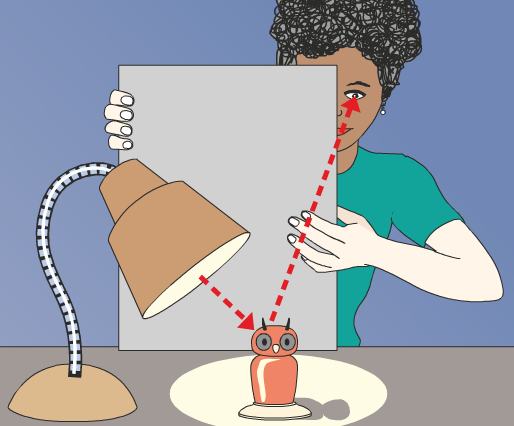
\includegraphics[scale=0.4]{bilan2}
	\end{center}
\end{frame}

\section{Voir la lumière}

\begin{frame}
	\begin{myact}{3 page 64}
	\begin{enumerate}\pause
		\item Dans une salle obscure, on ne voit pas la lumière entre le projecteur et le cône.\pause
		\item On observe une zone éclairée sur le cône.\pause
		\item Lorsque l'on saupoudre de la craie entre le projecteur et le cône on observe des grains de craie éclairés.\pause
		\item Si les grains ne sont pas dans la lumière, ils n'en reçoivent pas et ne sont donc pas visibles.\pause
		\item Dans cette expérience, les grains de craie sont des objets diffusants.\pause
		\item La lumière n'est visible que si on place des objets diffusants sur son trajet.
	\end{enumerate}
\end{myact}
\end{frame}


\begin{frame}
	\begin{mybilan}
	
	\twoCol{
	\begin{center}
		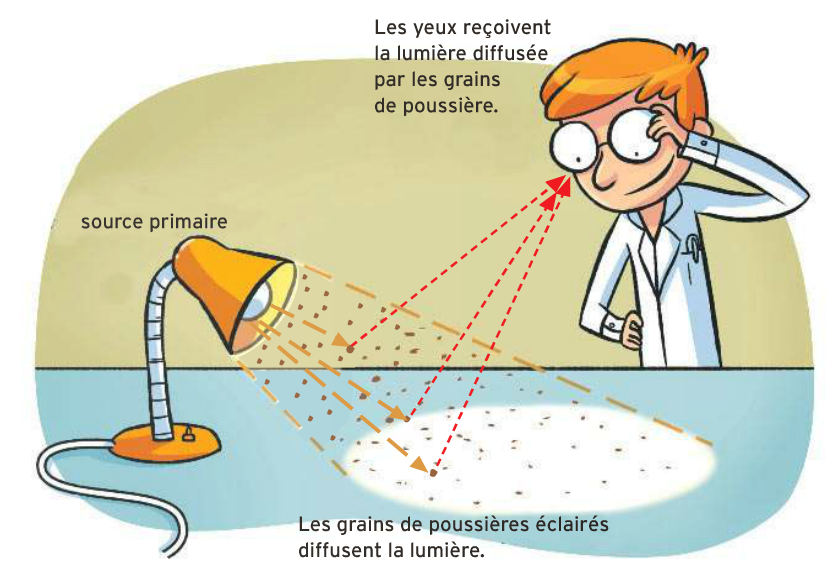
\includegraphics[scale=0.7]{bilan3}
	\end{center}

	\begin{itemize}
		\item Une tension est \kw{périodique} lorsque ses \kw{variations se répètent} identiques à elles mêmes au cours du temps. 
		\item La \kw{durée} d'un motif est la \kw{période}. On la note $T$, son unité est la seconde $s$.
	\end{itemize}
	}

\end{mybilan}
	
	\begin{center}
		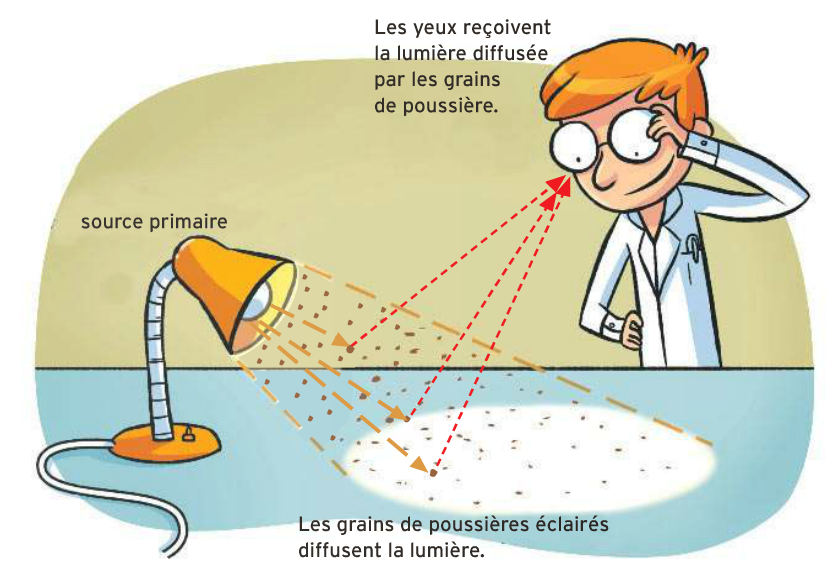
\includegraphics[scale=0.35]{bilan3}
	\end{center}
\end{frame}

%\section{Reconnaître le dioxyde de carbone}
%
%\begin{frame}
%	\begin{myact}{4 page 127}
	\begin{enumerate}
		\item Le gaz prélevé dans la seringue a été extrait d'eau pétillante par déplacement d'eau.\pause
		\item Au début de l'expérience, la solution d'eau de chaux est incolore et transparente.\pause
		\item Après y avoir fait barboter le gaz l'eau de chaux s'est troublée.\pause
		\item Un précipité blanc s'est formé lors de cette expérience, donc le gaz dissous dans l'eau pétillante est du dioxyde de carbone.
	\end{enumerate}
\end{myact}
%\end{frame}
%
%
%\begin{frame}
%	\begin{mybilan}
	\begin{itemize}
		\item La masse d'un corps est \kw{proportionnelle} à son volume; \pause
		\item Le coefficient de proportionnalité est la \kw{masse volumique} (notée $\rho$);\pause
		\item \kw{Un litre d'eau} a une masse de \kw{1 kilogramme};\pause
		\item Une substance est \kw{plus dense} qu'une autre si, pour un même volume, sa masse est supérieure.		
	\end{itemize}
\end{mybilan}
%\end{frame}

\end{document}